\problemname{Oreperations Research}
You run a massive mining facility that extracts ore from a mine and loads it onto long trains for shipment to factories around the nation. A train consists of $n$ cars, where car $i$ has capacity $c_i$, indicating how many tons of ore it can carry. Ore is dropped into the train cars at an overhead loading station from two separate queues of mine carts that run on either side the train. As with the train cars, mine carts hold varying loads of ore. Queue $A$ has $r$ carts, and cart $A_i$ carries a load of $a_i$. Similarly, queue $B$ has $s$ carts, and cart $B_i$ carries a load of $b_i$. Initially train car $1$ is at the loading station, and carts $A_1$ and $B_1$ are available to dump ore into it. The train car currently in the station can be given the load from the front cart in the $A$ queue, the front cart in the $B$ queue, or from both. If a cart doesn't dump its ore, it remains at the loading station; if it does dump its ore, it cycles back into the mine, loads up on ore, and rejoins the end of its queue. Meanwhile, the next cart in the queue moves into place and is available to dump ore.  Carts may not drop partial loads of ore and may not leave the loading station until they've emptied.  Similarly train cars may not be over-filled and may not leave the loading station until they are filled to capacity.  As soon as a train car is filled to capacity it leaves the loading station and the next train car pulls in. Your task is to determine whether given sequences of mine carts can be used to fill a given sequence of train cars to their capacity.

Figure~\ref{fig:ore1} shows an example of the process.  Here queue $A$ has three mine carts carrying loads $4$, $3$ and $2$, queue $B$ has four mine carts carrying loads $1$, $5$, $2$ and $2$, and the train has three cars with capacities $8$, $5$ and $4$.  The starting setup is shown in the leftmost image.  After (say) the first car in queue $A$ dumps its load into the first train car it goes back to the mine and (eventually) returns to the end of the line in queue $A$.  This situation is shown in the second image, where  the first train car still has capacity $4$ to be filled.  This can be accomplished by dumping ore from the front car of both queues $A$ and $B$. Once filled, the first train car moves out of the loading station leaving an alignment of cars and carts shown in the third image.  Here, the only way to fill the train car is for the front car of queue $B$ to dump its load.  This leads to the final image.  Here the last train car can be filled either by the front cars of both queues or the first two cars of queue $B$.  Note that if the third train car had capacity $3$ it could not be filled to full capacity.
\begin{figure}[!h]
\centering
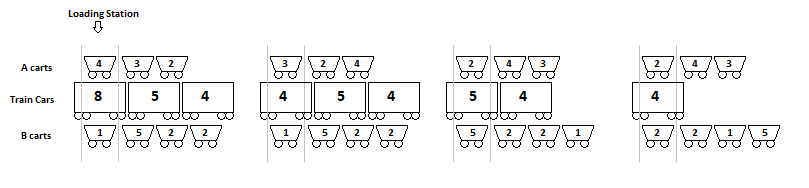
\includegraphics[width=0.9\textwidth]{ore1.png}
\caption{Sample Input $1$}
\label{fig:ore1}
\end{figure}

\section*{Input}
Input begins with a line containing three positive integers $r$ $s$ $n$ ($r,s \leq 50, n \leq 100)$ indicating the number of carts in queues $A$ and $B$ and the number of train cars, respectively. This is followed by three lines containing the values $a_1, a_2, \ldots, a_r$, $b_1, b_2, \ldots, b_s$, and $c_1, c_2, \ldots, c_n$, the capacities of the $A$ carts, the $B$ carts and the train cars, respectively.  The maximum capacity of any cart is $200$ and the maximum capacity of any train car is $2\,000\,000$. 

\section*{Output}
Output {\tt Yes} or {\tt No} indicating whether all of the train cars can be filled to capacity.
